\section{Approximations}
Our original definition of the derivative was motivated in part by finding the `best'
linear approximation to a curve at a given point. Indeed, if $ f $ is a function then,
for all $ h $ such that $ f(x_0 + h) $ is defined, we have
\begin{displaymath}
  f(x_0 + h) - f(x_0) = h f'(x_0) + \vartheta(h)
\end{displaymath}
where $ \lim_{h \to 0} \vartheta(h)/h = 0 $; in particular, for any $ x $ where $ f $
is defined (moreover, we need $ f $ to be defined everywhere \emph{between} $ x $ and $ x_0 $)
we have
\begin{displaymath}
  f(x) - f(x_0) = (x - x_0) f'(x_0) + \vartheta(x - x_0)
\end{displaymath}
where we have simply replaced $ h $ with $ x - x_0 $. We already defined the tangent
line to $ f $ at $ x_0 $ to be the line given by $ y - f(x_0) = (x - x_0) f'(x_0) $;
so the above equation tells us that if $ (x,y) $ is on the tangent line then
\begin{align*}
  f(x) - y = [(x - x_0) f'(x_0) + \vartheta(x - x_0) + f(x_0)] - [(x - x_0)f'(x_0) + f(x_0)] = \vartheta(x - x_0)
\end{align*}
and so we have that
\begin{displaymath}
  \frac{f(x) - y}{x - x_0} = \frac{\vartheta(x - x_0)}{x - x_0} \xrightarrow{x - x_0 \to 0} 0:
\end{displaymath}
in other words, as we move our point $ x $ of interest closer and closer to $ x_0 $, the `error' in
the tangent line approximation vanishes at a faster rate than our movement. Figure \ref{fig:approx1}
illustrates these relationships; notice that at points $ x $ close to the point of tangency (in this case $ x_0 = 2 $),
$ \tilde f(x) - f(x) $ is approaching zero faster than the distance $ \abs{x - x_0} $.

\begin{figure}
  \centering
  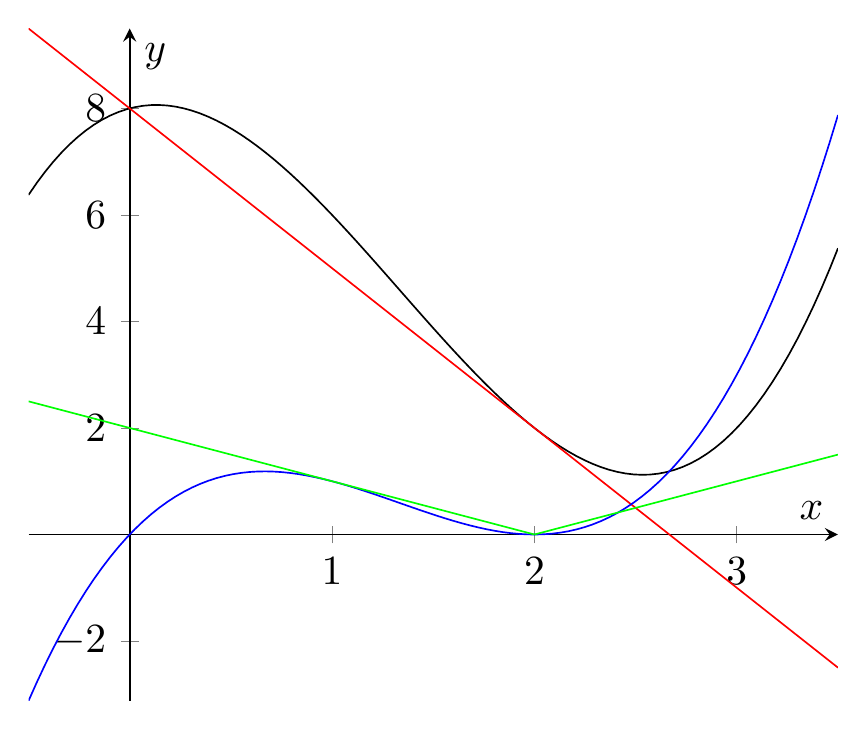
\begin{tikzpicture}[scale = 1.5]
    \begin{axis}[
      axis lines = center,
      xlabel = $ x $,
      ylabel = {$ y $},
    ] %(x -2)(x - 3) + (x + 1)(x - 3) + (x + 1)(x - 2) = x^2 - 5x + 6 + x^2 - 2x - 3 + x^2 - x - 2 = 3*16 - 2*16 + 1
      \addplot[domain = -0.5:3.5, color = black, samples = 100] {(x + 1)*(x - 2)*(x - 3) + 2};
      \addplot[domain = -0.5:3.5, color = red, samples = 5] {-3*(x - 2) + 2};
      \addplot[domain = -0.5:3.5, color = blue, samples = 100] {((x + 1)*(x - 2)*(x - 3) + 2) - (-3*(x - 2) + 2) };
      \addplot[domain = -0.5:2, color = green, samples = 5] { 2-x };
      \addplot[domain = 2:3.5, color = green, samples = 5] { x-2 };
    \end{axis}
  \end{tikzpicture}
  \caption{The graph of a function $ f(x) $ (black), its tangent line $ \tilde f(x) $ at $ 2 $ (red), $ f(x) - \tilde f(x) $ (blue), and $ y = \abs{x - 2} $ (green).\label{fig:approx1}}
\end{figure}

Given that the tangent line is, in this sense, a good linear approximation, it is natural to ask the following question:
\begin{center}\itshape
  If $ f $ is differentiable at $ x_0 $, what is the best polynomial approximation to $ f $ around the point $ x_0 $?
\end{center}

As a reminder, a polynomial is a function $ p $ of the form $ p(x) = p_n x^n + p_{n - 1} x^{n - 1} + \cdots + p_1 x + p_0 $
where $ p_n \neq 0 $. The various $ p_k $ are called the \emph{coefficients}, and $ n $ is the \emph{degree} of $ p $.

This question is an important one, because if we can answer it then we can always replace differentiable functions (which
are difficult to calculate --- what is $ \sin(32.341) $?) with polynomials (which only require a finite number of multiplications
and additions to calculate) with only a small loss of information.

Our plan of attack will be, given a function $ f $ that is differentiable (at least) $ n $ times at some point $ x_0 $,
to find a polynomial
\begin{displaymath}
  p(x) = p_n (x - x_0)^n + p_{n - 1} (x - x_0)^{n -1} + \cdots + p_1 (x - x_0) + p_0
\end{displaymath}
satisfying the following conditions:
\begin{align*}
  p(x_0) &= f(x_0)\\
  p'(x_0) &= f'(x_0)\\
  &\vdots\\
  p^{(n)}(x_0) &= f^{(n)}(x_0).
\end{align*}
(For convenience, the zeroth derivative of $ f $ is $ f $ itself.)

Our argument above shows that the linear polynomial approximation at $ x_0 $ is $ p(x) = f'(x_0)(x - x_0) + f(x_0) $. We will need the following lemma:

\begin{lemma}
  Let $ p(x) = p_n (x - x_0)^n + p_{n - 1} (x - x_0)^{n -1} + \cdots + p_1 (x - x_0) + p_0 $ be a polynomial. Then $ p_k = \frac{p^{(k)}(x_0)}{k!} $
  for all $ 0 \leq k \leq n $.
\end{lemma}
\begin{proof}
  We have the following:
  \begin{align*}
    p(x) = p_n (x - x_0)^n + \cdots + p_3 (x - x_0)^3 + p_2 (x - x_0)^2 + p_1 (x - x_0) + p_0 &\implies p(x_0) = p_0\\
    p'(x) = n p_n (x - x_0)^{n-1} + \cdots + 3p_3 (x - x_0)^2 + 2p_2 (x - x_0) + p_1 &\implies p'(x_0) = p_1\\
    p''(x) = n(n - 1) p_n (x - x_0)^{n - 2} + \cdots + (3 \cdot 2)p_2 (x - x_0) + 2p_2 & \implies p''(x_0) = 2p_2\\
    p^{(3)}(x) = n(n - 1)(n - 2) p_n (x - x_0)^{n - 3} + \cdots + (3 \cdot 2)p_2 & \implies p^{(3)}(x_0) = (2 \cdot 3)p_3\\
  \end{align*}
  and in general, completing the pattern,
  \begin{displaymath}
    p^{(k)}(x_0) = (k!)p_k.
  \end{displaymath}
\end{proof}

Thus, if we want to match $ f $ with a polynomial of degree $ n $ such that $ f^{(k)}(x_0) = p^{(k)}(x_0) $
for every $ 0 \leq k \leq n $ we simply choose $ p(x) = p_n (x - x_0)^n + p_{n - 1} (x - x_0)^{n -1} + \cdots + p_1 (x - x_0) + p_0 $
such that
\begin{displaymath}
  p_k = \frac{f^{(k)}(x_0)}{k!}.
\end{displaymath}
This polynomial is called the $ n$th \emph{Taylor polynomial} of $ f $ at $ x_0 $; we might even write $ \mathsf{T}_{n, x_0} f $
for this polynomial.

\begin{ex}0, 1, 0, -1, 0, 1,
  Consider $ f(x) = \sin x $. Then $ f^{(0)}(0) = 0 $, $ f^{(1)}(0) = 1 $, $ f^{(2)}(0) = 0 $, $ f^{(3)}(0) = -1 $, and in general
  \begin{displaymath}
    f^{(n)}(0) = \begin{cases*}
                   0 & $ n $ even\\
                   (-1)^{k} & $ n = 2k + 1 $ odd
                 \end{cases*}
  \end{displaymath}

  In particular, $ \mathsf{T}_{2k + 1, 0} f = x - \frac{1}{3!} x^3 + \frac{1}{5!} x^5 - \frac{1}{7!} x^7 + \cdots + \frac{(-1)^k}{(2k + 1)!}x^{2k + 1} $;
  the Taylor polynomials for $ k = 0 $ (red), $ k = 1 $ (green), and $ k = 2 $ (blue) are graphed in figure \ref{fig:approx2}.
  \begin{figure}
    \centering
    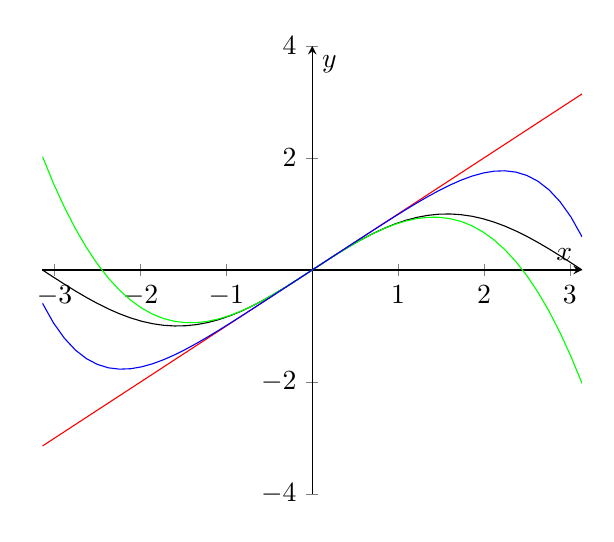
\begin{tikzpicture}
      \begin{axis}[
        axis lines = center,
        xlabel = $ x $,
        ylabel = {$ y $},
        ymax = 4,
        ymin = -4
      ]
        \addplot[domain = -pi:pi, color = black, samples = 50] { sin(deg(x)) };
        \addplot[domain = -pi:pi, color = red, samples = 50] { x };
        \addplot[domain = -pi:pi, color = green, samples = 50] { x - (1/6)*x^3 };
        \addplot[domain = -pi:pi, color = blue, samples = 50] { x - (1/120)*x^5 };
      \end{axis}
    \end{tikzpicture}
    \caption{The first few Taylor polynomials of sine.\label{fig:approx2}}
  \end{figure}
\end{ex}

We can even do the same error estimation that we performed above, although it is a little tedious; we
find that
\begin{equation}\label{eqn:tedious}
  \lim_{x \to x_0} \frac{f(x) - \mathsf{T}_{n, x_0} f(x)}{(x - x_0)^n} = 0
\end{equation}
(so $ \mathsf{T}_{n, x_0} \to f(x) $ faster than $ (x - x_0)^n \to 0 $).

Note that this only tells us that the Taylor polynomials $ \mathsf{T}_{n, x_0} f $ approximate $ f $ \emph{very, very, very} close to
the point $ x_0 $. It is not the case, in general, that the Taylor polynomials are a good approximation \emph{around} the point $ x_0 $.
For example, in one of the problems from the previous section we saw that
\begin{displaymath}
  f(x) = \begin{cases} e^{-1/x^2} & x \neq 0 \\ 0 &x = 0 \end{cases}
\end{displaymath}
is such that $ f^{(n)}(0) = 0 $ for all $ n $, and thus $ \mathsf{T}_{n, 0} f(x) = 0 $ for all $ n $; so even for large $ n $, the Taylor
polynomials are a terrible approximation!


\subsection{Exercises and Problems}
\begin{enumerate}
  \item Find the best quadratic approximation to $ f(x) = 1/(1 + x^2) $ at zero.
  \item Find the first, second, third, and $ n$th Taylor polynomials of the following functions at zero.
    \begin{enumerate}
      \item $ x \mapsto e^x $
      \item $ x \mapsto \cos x $
      \item $ x \mapsto \frac{1}{1 + x} $
    \end{enumerate}
  \item
    \begin{enumerate}
      \item According to problem set 6 of the trigonometry notes (remember those!), $ \arctan a + \arctan b = \arctan \left[(a + b)/(1 - ab)\right] $
            as long as the sum on the left is between $ \pm \pi/2 $. Show that $ \pi/4 = 5\arctan (1/5) - \arctan(1/239) $.
      \item Show that $ \pi = 3.14159... $.
    \end{enumerate}
  \item
    \begin{enumerate}
      \item Let $ p(x) $ be a polynomial of degree $ n $, and let $ x_0 $ be any point. Show that for all $ x $, $ p(x) = \mathsf{T}_{n, x_0} p(x) $.
      \item Write the function $ p(x) = 22 - 49 x + 35 x^2 - 10 x^3 + x^4 $ as a polynomial in $ (x-3) $.
    \end{enumerate}
  \item Suppose $ f $ and $ g $ both have $ n $ derivatives at $ x_0 $. Let $ \lambda $ be a real number. Calculate:
    \begin{enumerate}
      \item $ \mathsf{T}_{n, x_0} (\lambda f) $
      \item $ \mathsf{T}_{n, x_0} (f + g) $
      \item $ \mathsf{T}_{n, x_0} (fg) $
      \item $ \mathsf{T}_{n-1, x_0} (f') $
    \end{enumerate}
  \item Prove formula \ref{eqn:tedious} above.
\end{enumerate}

\subsection{References}
An introduction to the approximation of sufficiently differentiable functions by polynomials can be found
in Spivak, chapter 19. With a little extra work one can work out what degree of polynomial is needed at a
point $ x_0 $ to reduce the error to less than a specified amount; to do this one needs integration (which
we have not yet seen), and the details are in Spivak.

\subsection{Homework problems}
\begin{enumerate}
  \item Find the best quartic (degree 4 polynomial) approximation to $ f(x) = x^5 + x^3 + x $ about (a) 0 and (b) 1.
  \item Square roots are difficult. Compute an approximation to $ \sqrt{4.003} $ by hand. (Hint: expand $ x \mapsto \sqrt{x} $ as a Taylor series about 4.)
\end{enumerate}
